%%%%%%%%%%%%%%%%%%%%%%%%%%%%%%%%%%%%%%%%%
% Focus Beamer Presentation
% LaTeX Template
% Version 1.0 (8/8/18)
%
% This template has been downloaded from:
% http://www.LaTeXTemplates.com
%
% Original author:
% Pasquale Africa (https://github.com/elauksap/focus-beamertheme) with modifications by 
% Vel (vel@LaTeXTemplates.com)
%
% Template license:
% GNU GPL v3.0 License
%
% Important note:
% The bibliography/references need to be compiled with bibtex.
%
%%%%%%%%%%%%%%%%%%%%%%%%%%%%%%%%%%%%%%%%%

%----------------------------------------------------------------------------------------
%	PACKAGES AND OTHER DOCUMENT CONFIGURATIONS
%----------------------------------------------------------------------------------------

\documentclass{beamer}

\usetheme{focus} % Use the Focus theme supplied with the template
% Add option [numbering=none] to disable the footer progress bar
% Add option [numbering=fullbar] to show the footer progress bar as always full with a slide count

% Uncomment to enable the ice-blue theme
%\definecolor{main}{RGB}{92, 138, 168}
%\definecolor{background}{RGB}{240, 247, 255}

%------------------------------------------------

\usepackage{booktabs} % Required for better table rules

\usepackage[brazilian]{babel}
\usepackage[utf8]{inputenc}
\usepackage[T1]{fontenc}

%----------------------------------------------------------------------------------------
%	 TITLE SLIDE
%----------------------------------------------------------------------------------------

\title{Diagnóstico do Glaucoma Usando Imagens de Espessura da Camada de Fibras Nervosas}

% \subtitle{VII Workshop de Pós-Graduação - Engenharia da Computação - WPGEC 2018}

\author{Samira J. Braga \\ Edson S. Gomi}

% \titlegraphic{\includegraphics[scale=1.25]{Images/focuslogo.pdf}} % Optional title page image, comment this line to remove it

\institute{Escola Politécnica da Universidade de São Paulo}

\date{22/11/2018}

%------------------------------------------------

\begin{document}

%------------------------------------------------

\begin{frame}
	\maketitle % Automatically created using the information in the commands above
\end{frame}

%----------------------------------------------------------------------------------------
%	 SECTION 1
%----------------------------------------------------------------------------------------

% \section{Objetivos e motivação} % Section title slide, unnumbered

%------------------------------------------------

\begin{frame}{Glaucoma}
    Glaucoma é uma doença crônica que caracteriza-se pela perda da camada de fibras nervosas no olho. Se não tratada pode  levar  à  cegueira  irreversível.
    \vfill
    \begin{columns}
		\column{0.5\textwidth}
        O  diagnóstico  do  glaucoma  é  feito  com  uma combinação  de  exames de OCT e perimetria  computadorizada. Muitas vezes é necessária a avaliação de um especialista. 
		
        \column{0.5\textwidth}
            \begin{figure}
                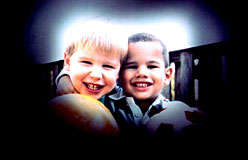
\includegraphics[width=\linewidth]{img/glaucomavision.jpg} 
                \caption{Visão de uma pessoa com glaucoma}
            \end{figure}
            
            
    \end{columns}
    
\end{frame}

\begin{frame}{Redes Neurais Convolucionais}

    \begin{figure}
        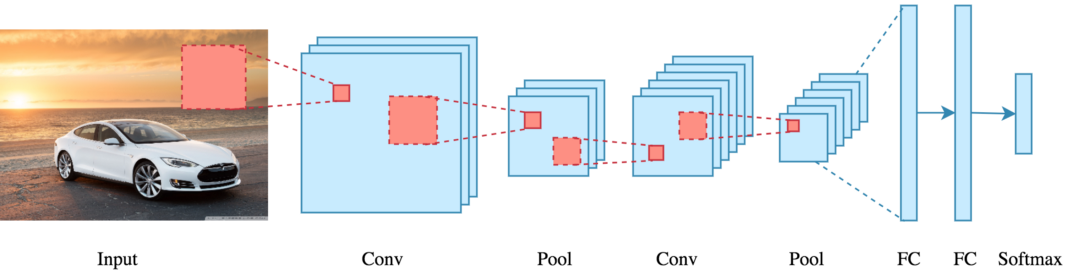
\includegraphics[width=\linewidth]{img/convolucao.png} 
        \caption{Esquema de uma rede neural convolucional}
    \end{figure}
    
\end{frame}

\begin{frame}{Transfer Learning}
    Usar uma rede treinada com um dataset grande de imagens em  um  domínio  mais  amplo  e  transferir  esse  conhecimento para  um  domínio  mais  específico.
    Li et al obteve bons resultados na classificação de retinopatia diabética utilizando transfer learning [2]. No trabalho de Lee et al, a rede VGG16 foi utilizada para classificar degeneração macular em imagens de tomografia de coerência óptica [3].
    
\end{frame}

\begin{frame}{Objetivo}

    O objetivo deste trabalho é investigar se é possível fazer o diagnóstico a partir das imagens da espessura da camada de fibras nervosas do olho por meio de uma rede neural convolucional (CNN).
    
\end{frame}

\begin{frame}{Experimento}
    
    \begin{itemize}
        \item Rede VGG16
        \item Classificação de pacientes em glaucoma e normal
        \item Imagens de espessura de camada de fibras nervosas
        \item Utilização de técnica de transfer learning
        \item 9800 imagens no dataset de treinamento
        \item 24 imagens no dataset de validação
        \item Framework de deep learning utilizado: Caffe
    \end{itemize}
    
\end{frame}

\begin{frame}{Resultados}
    \begin{columns}
		\column{0.5\textwidth}
            \begin{itemize}
                \item Acurácia final de 95.8\%
                \item 5000 iterações
                \item 1h de processamento
            \end{itemize}
		
        \column{0.5\textwidth}
            \begin{figure}
                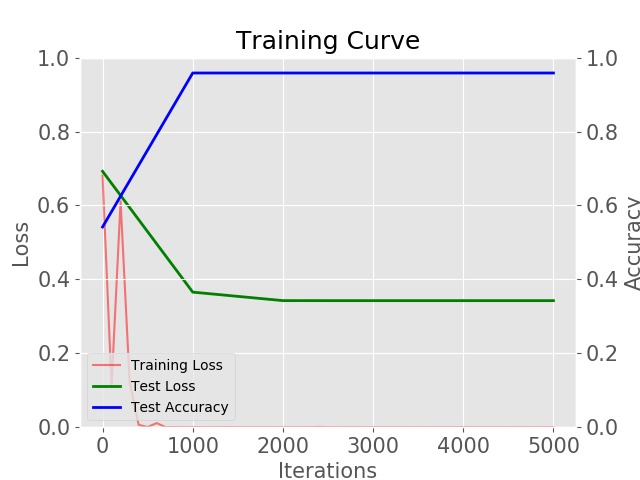
\includegraphics[width=\linewidth]{img/curve_vgg16.png}
                \caption{Evolução de acurácia e erro de treino e validação} 
            \end{figure}            
            
    \end{columns}
    
\end{frame}

\begin{frame}{Conclusão}
    \begin{itemize}
        \item Diagnóstico de glaucoma a partir de imagens de OCT é viável
        \item Resultados até o momento mostram alto erro no dataset de validação
        \item Possível ocorrência de overfitting devido à pequena quantidade de imagens no dataset de treino
    \end{itemize}
\end{frame}

\begin{frame}[focus]
	Obrigada pela atenção \\ Perguntas?
\end{frame}

% \section{CNNs em oftalmologia}

% \section{Metodologia e desenvolvimento}



\end{document}
